\documentclass[12pt,letterpaper]{article}
%\documentclass[12pt,letterpaper,draft]{article}
%\documentclass[12pt,a4paper]{article}
\usepackage[cp866]{inputenc}
\usepackage[T1]{fontenc}
%\usepackage[T2C]{fontenc}
\usepackage[full]{textcomp}
\usepackage{calc}
\usepackage{array}
\usepackage{amsmath,amssymb}
%\usepackage[english,russian]{babel}
\usepackage[english,russian]{babel}

\usepackage{pxfonts}

\usepackage{examplep}
%\usepackage[scaled]{luximono}
%\usepackage{lucida}
\usepackage[scaled]{helvet}
%\usepackage{courier}
%\usepackage[boldsans]{ccfonts}
\usepackage[euler-digits]{eulervm}
%\usepackage{ragged2e}
\usepackage{color}
\usepackage{tabularx}
%\usepackage{tabulary}
\usepackage{paralist}
\usepackage{xspace}
%\usepackage{layout}
%\usepackage[paper=letterpaper,hoffset=-0.5in,voffset=-0.5in,textwidth=474pt,textheight=628pt,heightrounded=true]{geometry}
%\usepackage[top=1in, left=1in, right=1in, bottom=1in, includefoot, heightrounded=true]{geometry}
\usepackage[paper=letterpaper, top=1in, left=1in, right=1in, bottom=1in, includefoot, heightrounded=true]{geometry}
\usepackage{fancyvrb}
%\usepackage{listings}
\usepackage{fancyhdr}

\pagestyle{fancy}
\setlength\headheight{15pt}
\renewcommand\sectionmark[1]{\markboth{#1}{}}
\renewcommand\subsectionmark[1]{\markright{\thesubsection\ #1}}
\definecolor{darkgreen}{rgb}{0,0.5,0}
\definecolor{darkblue}{rgb}{0,0,0.5}
\renewcommand\tabularxcolumn[1]{>{\small}m{#1}}
%\newcolumntype{Y}{>{\vphantom{$\big|$}\raggedright\arraybackslash}X}
\newcolumntype{Y}{>{\raggedright\arraybackslash}X}

\VerbatimFootnotes
\renewcommand{\FancyVerbFormatLine}[1]{\textcolor{darkblue}{#1}}

\newif\ifpdf
    \ifx\pdfoutput\undefined
        \pdffalse % we are not running PDFLaTeX
    \else
        \pdfoutput=1 % we are running PDFLaTeX
    \pdftrue
    \fi

\ifpdf
    \usepackage[pdftex]{graphicx}
    \pdfcompresslevel=9
    \pdfpkresolution=1200
    \pdfdecimaldigits=3
    \pdfuniqueresname=1     % positive value turns on preceding unique
                            % prefix for each named resources
\else
    \usepackage[dvips]{graphicx}
\fi

\newcommand{\URL}[2]{%
    \pdfstartlink attr{/Border [0 0 0]} user{%
    /Subtype /Link
    /A <<
        /Type /Action
        /S /URI
        /URI (#2)
    >>}%
\textcolor{blue}{#1}%
\pdfendlink}

\newcommand{\GO}[2]{%
\pdfstartlink attr{/Border [0 0 0]}%
goto name{#2}%
\textcolor{darkgreen}{#1}%
\pdfendlink}

\newcommand{\GOT}[2]{%
\pdfstartlink attr{/Border [0 0 0]}%
goto name{#2}%
\textcolor{darkgreen}{\texttt{#1}}%
\pdfendlink}

\newcommand{\FORTRAN}{\textsf{FORTRAN}\xspace}
\newcommand{\TildaT}{\usefont{T1}{ul9}{m}{n}{\symbol{3}}}
\newcommand{\Tilda}{\symbol{3}\xspace}
\newcommand{\conj}{\operatorname{conj}}
\newcommand{\floor}{\operatorname{floor}}
\newcommand{\pinv}{\operatorname{pinv}}
\newcommand{\CVMVERSION}{8.1\xspace}
\newcommand{\MKLVERSION}{11.1 Update~1\xspace}
\newcommand{\ACMLVERSION}{4.4.0\xspace}
\newcommand{\ACMLVERSIONSIXFOUR}{5.3.0\xspace}
\newcommand{\Based}{\GO{$\ell$-based}{SubSubSectionIndexing}\xspace}


%\newcommand{\CodeB}[1]{\textcolor{darkblue}{\texttt{#1}}}
\newcommand{\Code}[1]{\texttt{#1}}

\makeatletter
\renewcommand\section{\@startsection {section}{1}{0mm}%
                                   {-3.5ex \@plus -1ex \@minus -.2ex}%
                                   {2.3ex \@plus.2ex}%
                                   {\normalfont\Large\bfseries\sffamily}}
\renewcommand\subsection{\@startsection{subsection}{2}{0mm}%
                                     {-3.25ex\@plus -1ex \@minus -.2ex}%
                                     {1.5ex \@plus .2ex}%
                                     {\normalfont\large\bfseries\sffamily}}
\renewcommand\subsubsection{\@startsection{subsubsection}{3}{0mm}%
                                     {-3.25ex\@plus -1ex \@minus -.2ex}%
                                     {1.5ex \@plus .2ex}%
                                     {\normalfont\normalsize\bfseries\sffamily}}
\makeatother

\allowdisplaybreaks

%%%%%%%%%%%%%%%%%%%%%%%%%%%%%%%%%%%%%%%%%%%%%%%%%%%%%%%%%%%%%%%%%%%%%%%%
\begin{document}

\selectlanguage{english}

%\renewcommand{\thefootnote}{\fnsymbol{footnote}}

\section{Preface}
\subsection{Brief history}
CVM%
\pdfdest name {SectionPreface} fit%
\pdfdest name {SubSectionBriefHistory} fit{}
C++ class library%
\footnote{\,This document describes version \CVMVERSION and it does not cover function classes yet. 
Use online documentation for them. Copyright
\copyright{ } Sergei Nikolaev, 1992--2012,
\URL{http://cvmlib.com}{http://cvmlib.com}} encapsulates
concepts of vector and different kinds of matrices including square,
band, symmetric and hermitian ones, in Euclidean space of real and
complex numbers.
The library is distributed under the \URL{Boost Software License, Version~1.0}{http://www.boost.org/LICENSE_1_0.txt}.
First version of the library was released in 1992.
Originally it allowed to simplify a code dealing with matrices and
vectors in the following way:
\begin{Verbatim}
rvector a(10), b(20);
rmatrix A(20,10);
......
b = A * a;
cout << "Norm of b equals " << b.norm() << endl;
\end{Verbatim}
By overloading of arithmetic operators and parentheses relative
readability of source code was achieved.

In 1995\footnote{\,I'm not sure actually, may be that was 1994}
Russian office of Intel Corporation began to distribute a CD with
last software products from Intel. Among others there was a freely
(at that time) distributed library called ``Intel BLAS Library''.
More than 20 years \URL{BLAS library}{http://www.netlib.org/blas}
(Basic Linear Algebra Subprograms) is known to experts in numerical
algorithms programming in \FORTRAN language. This library features
common vector-matrix operations for data types \verb"REAL" and
\verb"DOUBLE RECISION". 
%It's important to note here that CVM
%library is also released in two versions:
%\begin{Verbatim}
%#if defined (CVM_FLOAT)
%    typedef float treal;
%#else
%    typedef double treal;
%#endif
%\end{Verbatim}
Both implementations of the BLAS are utilized since version 2.0 of
CVM library. For example, operator of addition of two vectors
utilizes subroutine \verb"DAXPY". Later Intel changed the name
``BLAS'' to ``Intel Math Kernel Library''. Since version 3.0
\URL{LAPACK}{http://www.netlib.org/lapack} subroutines were
added to the Intel MKL library.
% This functionality was encapsulated in third release of the CVM library. 
Version 4.0 featured complex numbers. And since version
5.0 band, symmetric and hermitian matrices are implemented as well.
Version~6.0 had many additional algorithms implemented, performance 
enhancements and bug fixes. Version~6.1 brought transposed versions of 
linear solvers as well some vec\-tor--matrix operators.
Version~7.0 added functional classes including elementary functions,
vectors and matrices of them and supporting simplification and
derivatives computation (analytically, not numerically).
Version~8.0 implemented new C++~11 standard features like move semantics 
for better performance.

\subsection{Libraries Supported}
The
\URL{last version}{http://developer.intel.com/software/products/mkl/} of the
Intel MKL library at the moment of writing of this document for Win32 and
Linux is \MKLVERSION. Version~\CVMVERSION of the CVM library was 
built and tested with that MKL library implementation.

Besides that \URL{AMD ACML library}{http://developer.amd.com/cpu/Libraries/acml/Pages/default.aspx}
is supported as well. Current CVM Library was 
built and tested with AMD ACML~\ACMLVERSION for 32 bit plaforms 
and ACML~\ACMLVERSIONSIXFOUR for 64~bit.

Finally, \URL{native BLAS and LAPACK}{http://www.netlib.org/lapack/} libraries
are supported and starting from CVM 5.7 they are part of binary packages as well.


\subsection{Object Model}
Object%
\pdfdest name {SubSectionTheModel} fit{}
model of the CVM library is shown on the following picture\\
\noindent
%\begin{figure}
\unitlength=1mm
\begin{picture}(130,160)(0,0)
\put(-23,-121){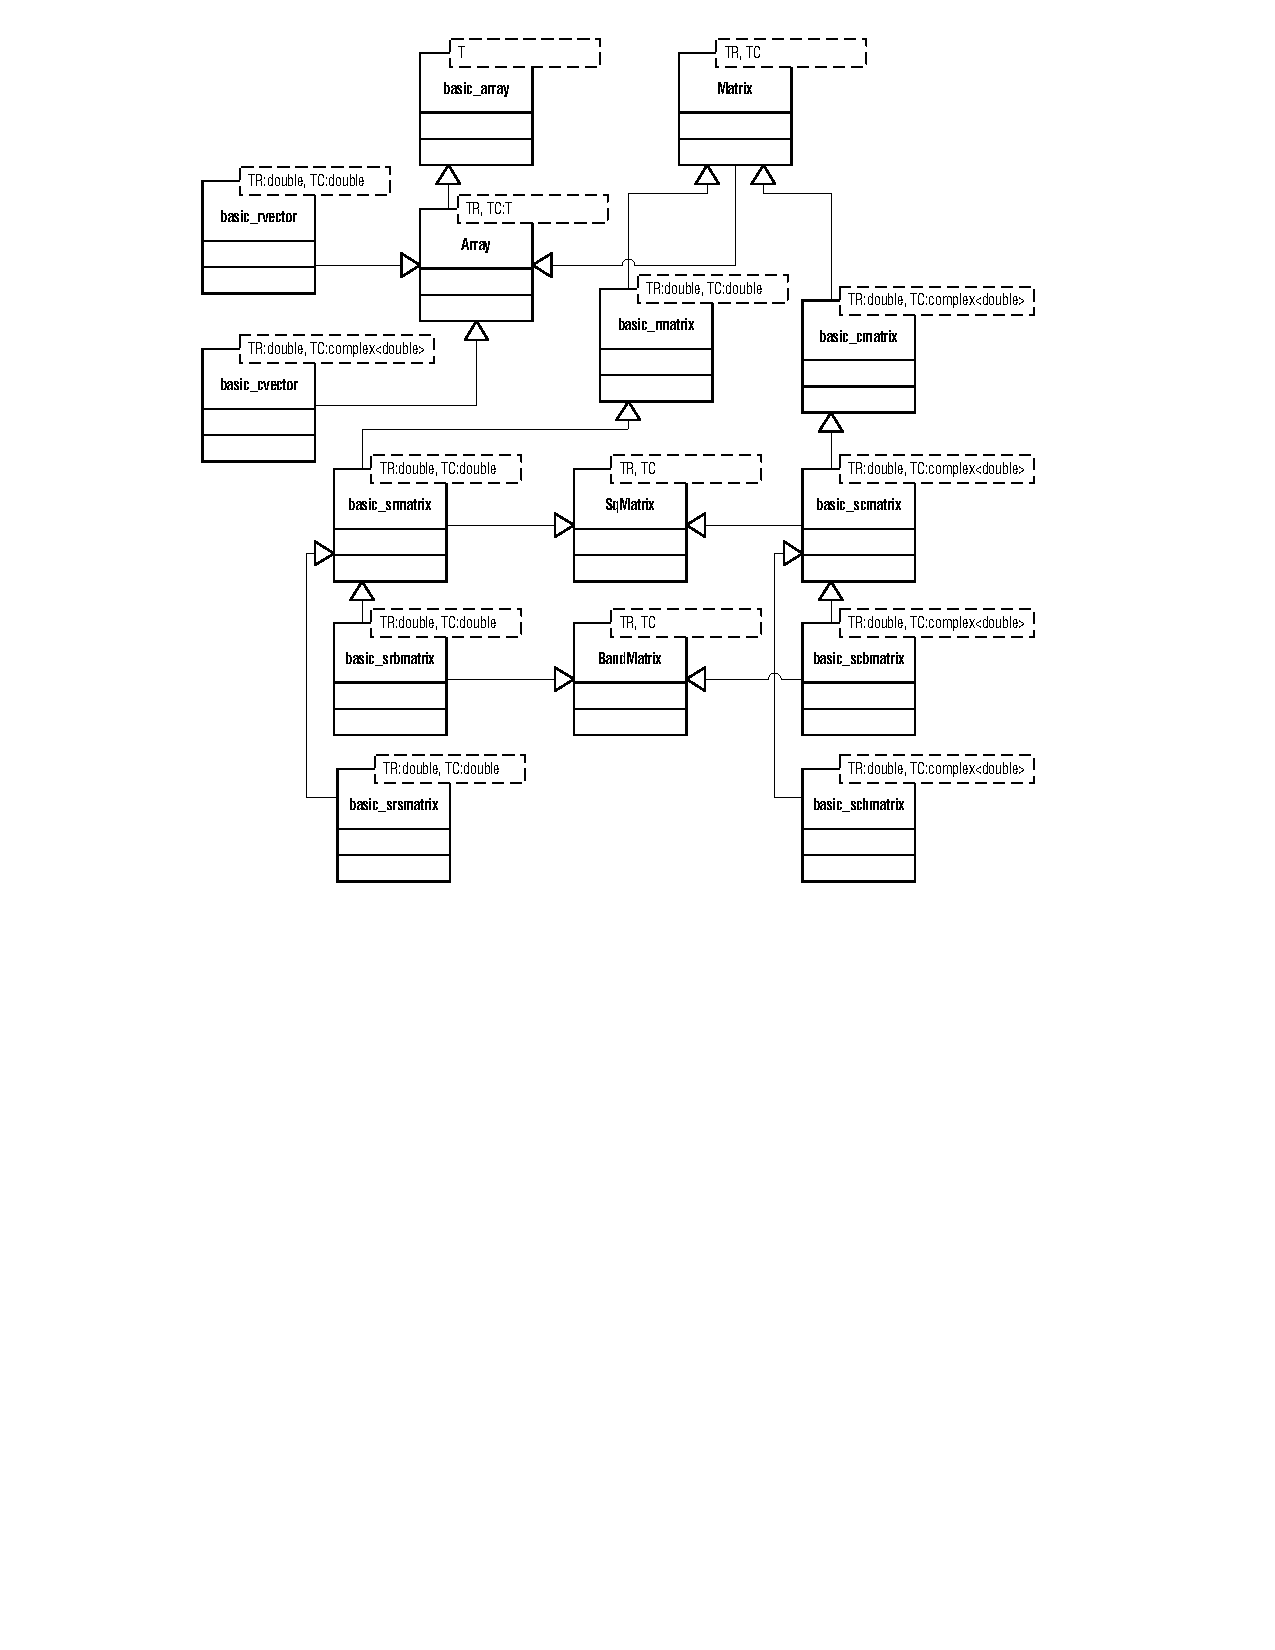
\includegraphics[width=215mm]{model.pdf}}
\end{picture}
%\end{figure}
\unitlength=1pt
%\newpage

Base class's names are beginning with capital letters. They
implement common interfaces and are \emph{not} designed to be instantiated.
This is the list of end-user classes:
\begin{compactitem}
\item \verb"basic_array" is an abstract array of elements of any type.
It's used
mostly as an array of integers like \verb"basic_array<int>", but you
can use it in your projects within any other types as well.
\item \verb"basic_rvector" is a class encapsulating vector
of real numbers.
\item \verb"basic_cvector" is a class encapsulating vector
of complex numbers.
\item \verb"basic_rmatrix" is a class encapsulating matrix
of real numbers.
\item \verb"basic_cmatrix" is a class encapsulating matrix
of complex numbers.
\item \verb"basic_srmatrix" is a class encapsulating 
square matrix of real numbers.
\item \verb"basic_scmatrix" is a class encapsulating 
square matrix of complex numbers.
\item \verb"basic_srbmatrix" is a class encapsulating 
square band matrix of real numbers. Packed storage is
used.
\item \verb"basic_scbmatrix" is a class encapsulating 
square band matrix of complex numbers. Packed storage
is used.
\item \verb"basic_srsmatrix" is a class encapsulating 
symmetric matrix of real numbers.
\item \verb"basic_schmatrix" is a class encapsulating 
hermitian matrix of complex numbers.
\end{compactitem}

You don't need to use those class names directly unless you
want to \verb"typedef"
your own ones. Otherwise you should use the following
pre-defined classes:
%(\verb"CVMAllocator" is omitted here for simplicity):
\begin{Verbatim}
typedef basic_array    <int>             iarray;
typedef basic_rvector  <treal>           rvector;
typedef basic_rmatrix  <treal>           rmatrix;
typedef basic_srmatrix <treal>           srmatrix;
typedef basic_cvector  <treal, tcomplex> cvector;
typedef basic_cmatrix  <treal, tcomplex> cmatrix;
typedef basic_scmatrix <treal, tcomplex> scmatrix;
typedef basic_srbmatrix<treal>           srbmatrix;
typedef basic_scbmatrix<treal, tcomplex> scbmatrix;
typedef basic_srsmatrix<treal>           srsmatrix;
typedef basic_schmatrix<treal, tcomplex> schmatrix;
\end{Verbatim}
The rest of this manual describes them in details.




\subsection{Installation}
\subsubsection{Directory Structure}
The%
\pdfdest name {SubSectionInstallation} fit{}
CVM%
\pdfdest name {SubSubSectionDirectoryStructure} fit{}
library distribution has the following directory structure.
\begin{compactitem}
\item \verb".\*2010.sln" MS Visual~Studio~2010 solution files.
\item \verb".\*2012.sln" MS Visual~Studio~2012 solution files.
\item \verb"ftn" contains \FORTRAN{} files.
%for Intel Fortran compiler and GNU \verb'gfortran'. 
This source code
is the part of CVM library, it contains some
numerical algorithms implementation.
\item \verb"lib" is the place for 32-bit libraries.
\item \verb"lib64" is the place for 64-bit libraries.
\item \verb"test" contains regression test code and projects.
\item \verb"src" contains source code of the library
along with \verb"cvm.h" header file.
\end{compactitem}



\subsubsection{Usage Notes}
These%
\pdfdest name {SubSubSectionUsageNotes} fit{}
are definitions and data types used in the library.\\
\phantom{1em}\\
\begin{tabularx}{\textwidth}{|r|Y|} \hline
%\vphantom{$\big|$}
%\begin{tabular}{|>{\raggedleft\hspace{0pt}}m{4cm}|>{\raggedright\hspace{0pt}}m{\linewidth-4cm}|} \hline
\Code{CVM\_ZERO\_BASED} & define this macro to build the library with \GO{$0$-based indexing}{SubSubSectionIndexing}
\\ %tabularnewline
\hline
\Code{CVM\_ACML} & define this macro to link against AMD ACML and/or ACML MP library
\\ %tabularnewline
\hline
\Code{CVM\_FLOAT} & define this macro in order to build a float version
\\ %tabularnewline
\hline
\Code{CVM\_NO\_NAMESPACE} & define this macro
if you don't want to use namespace
\\ %tabularnewline
\hline
\Code{tint} & is \Code{typedef}'ed as \Code{long long int} (or as \Code{\_\_int64} for MSVC)
if \Code{ILP64} is defined and as \Code{int} otherwise (by default)
\\ %tabularnewline
\hline
\Code{treal} & is \Code{typedef}'ed as \Code{float}
if \Code{CVM\_FLOAT} is defined and as \Code{double} otherwise (by default)
\\ %tabularnewline
\hline
\Code{tcomplex} & is \Code{typedef}'ed as
\Code{std::complex<treal>}
\\ %tabularnewline
\hline
%\Code{CVM\_ALLOCATOR} & assign this macro to a name of your own \GO{allocator}{SubSubSectionAllocator} in order to rebuild CVM class library
%\\ %tabularnewline
%\hline
\end{tabularx}
\phantom{1em}\\
In order to use the library just include its header file:
\begin{Verbatim}
#include <cvm.h>
\end{Verbatim}
You should also link your project with one of \verb"cvm*.lib"
for Microsoft's C++ compilers
and \verb"cvm*.so" for GNU~C++ compilers
(debug versions are \verb"*_debug.lib" and \verb"*_debug.so"
respectively).

\subsubsection{Installation -- Win32}
If%
\pdfdest name {SubSubSectionInstallationWin32} fit{}
you don't want to rebuild the library just download
an appropriate version of \verb"cvm*.dll" and \verb"cvm*.lib" files
from binaries section.
If you want to rebuild the whole library you'll
need Intel Fortran~11.1 and Intel C++~11.1 compilers (or higher)
along with MS~Visual~Studio~2010 or 2012.
You'll also need
the Intel MKL~10.2 (or higher) library.
You will also need STL library 
coming with MS~VC++ or
the \URL{STLport}{http://stlport.com} library.
Open \verb".\cvmlib*.sln" solution
and choose the library version you want to build.

%\setlength\extrarowheight{3pt}

%\subsubsection{Dependencies -- Win32}
%There is no external dependencies anymore. Everything is linked into
%the binaries distributed within the library (including those Intel's
%runtime .so files for Linux).


\subsubsection{Installation -- Unix and MinGW}
Use%
\pdfdest name {SubSubSectionInstallationUnix} fit{}
the Makefile provided in the root directory:
\begin{Verbatim}
make [release|debug] [IFORT=1] [ICC=1] [MKL=1] [MKL_PATH=/opt/...] 
     [ACML=1] [ACML_MP=1] [ACML_PATH=/opt/...] [EM64T=1] [ILP64=1]
     [CVM_FLOAT=1] [ICCT=1] [STATIC_ONLY=1] [IFORT_PATH=/opt/...] 
     [MAC=1]
\end{Verbatim}
Here
\begin{compactitem}
\item \verb'release|debug' is a target (by default it builds both)
\item \verb'IFORT=1' instructs to use \verb"ifort"
%Intel~Fortran 
compiler (by default it's \verb'gfortran')
\item \verb'ICC=1' instructs to use \verb"icpc"
%Intel~C++ compiler 
(by default it's \verb'g++')
\item \verb'MKL=1' instructs to use Intel~MKL library (by default it uses
  native BLAS and LAPACK libraries)
\item \verb'MKL_PATH=path' specifies the directory where the~MKL is installed to.
By default it's equal to \verb'/opt/intel/composerxe/mkl/lib'.
%(please make sure that this path contains \verb'32' and \verb'em64t' subdirectories inside).
\item \verb'ACML=1' instructs to use AMD ACML library (overrides \verb'MKL=1' and \verb'ACML_MP=1').
\item \verb'ACML_MP=1' instructs to use AMD ACML MP library (overrides \verb'MKL=1').
\item \verb'ACML_PATH=path' specifies the directory where the ACML is 
installed to.
(overrides \verb'MKL_PATH=path').
\item \verb'EM64T=1' instructs to build EM64T version of the library.
\item \verb'ILP64=1' instructs to build INT64-based version of the library (EM64T must be turned on).
\item \verb'CVM_FLOAT=1' instructs to build \verb'float' version of the
  library.
\item \verb'ICCT=1' instructs to use Intel~C++ compiler for building the
regression test utility (by default it's \verb'g++')
\item \verb'STATIC_ONLY=1' instructs to build static libraries only.
Both .so and .a will be built otherwise.
\item \verb'IFORT_PATH=path' specifies the directory where the Intel Fortran is installed to. 
It's required only when you build ACML version within Intel Fortran and
Intel C++ compilers.
\item \verb'MAC=1' instructs to build Mac OS X version of the library.
\end{compactitem}
On Unix platforms Intel~MKL, AMD ACML and native BLAS/LAPACK libraries as well
as both Intel's and GNU compilers are supported. On MinGW platform the native libraries and
compilers are only supported.


\subsection{Storage}
The%
\pdfdest name {SubSubSectionStorage} fit{}
way of storage of matrices units is the same as the \FORTRAN's one.
Units are stored by columns, see the following example:
\begin{Verbatim}
cvm::rmatrix m(2,2);
m(1,1) = 1.;       // first  row, first  column
m(1,2) = 2.;       // first  row, second column
m(2,1) = 3.;       // second row, first  column
m(2,2) = 4.;       // second row, second column
double* p = m;
cout << p[0] << " " << p[1] << " " << p[2] << " " << p[3] << endl;
\end{Verbatim}
Output will be the following:
\begin{Verbatim}
1 3 2 4
\end{Verbatim}
Since version 5.0 band matrices are introduced. Band storage can be
described as follows (cited from MKL manual): \textit{%
an $m$ by $n$ band matrix with $k_l$ sub-diagonals and $k_u$ super-diagonals is stored
compactly in a two-dimensional array with $k_l+k_u+1$ rows and $n$ columns. Columns of the
matrix are stored in the corresponding columns of the array, and diagonals of the matrix are
stored in rows of the array}. This way of storage can be illustrated as follows
%(here $m=n=6$, $k_l=1$, $k_u=2$ in first case and
%$m=n=3$, $k_l=0$, $k_u=0$ in second case),
(referenced elements are shown as ``$*$'', not referenced as ``$-$'', zeros are not stored):
\begin{align*}
m=n=3, k_l=0, k_u=0&:\ \begin{bmatrix}
* & 0 & 0 \\
0 & * & 0 \\
0 & 0 & *
\end{bmatrix}\\
%\end{align*}
%\begin{align*}
m=n=4, k_l=1, k_u=0&:\ \begin{bmatrix}
* & 0 & 0 & 0 \\
* & * & 0 & 0 \\
0 & * & * & 0 \\
0 & 0 & * & * \\
  &   &   & -
\end{bmatrix}\\
m=n=6, k_l=1, k_u=2&:\ \begin{bmatrix}
- &   &   &   &   &   \\
- & - &   &   &   &   \\
* & * & * & 0 & 0 & 0 \\
* & * & * & * & 0 & 0 \\
0 & * & * & * & * & 0 \\
0 & 0 & * & * & * & * \\
0 & 0 & 0 & * & * & * \\
0 & 0 & 0 & 0 & * & * \\
  &   &   &   &   & -
\end{bmatrix}
\end{align*}
CVM library implements square band matrices only,
therefore $m=n$ is satisfied for them.


\subsection{Indexing}
By default index%
\pdfdest name {SubSubSectionIndexing} fit{}
numbering in CVM library
corresponds to the \FORTRAN's one: index of the
first unit is equal to $1$:
\begin{Verbatim}
cvm::rector v(2);
cvm::rmatrix m (2,3);
v[1] = 1.3;       // first vector unit
v(2) = 2.1;       // second vector unit
m(1) = v;         // first column of matrix
m(1,2) = 3.7;     // element located on the first row
                  // and the second column of matrix
\end{Verbatim}
Starting from version 5.7 $0$-based indexing is supported as well.
In order to use it you'd need to re-build the library with
\Code{CVM\_ZERO\_BASED} macro defined. 
To distinguish this fact, \Based notation 
will be used below in this document, which means $1$-based by default
and $0$-based if the macro is used.


\subsection{Polymorphism}
The%
\pdfdest name {SubSectionPolymorphism} fit{}
majority of CVM Class Library member functions are not declared
as virtual, but it doesn't mean that the classes are not polymorphic.
Those member functions just wrap virtual ones. For example,
the following code
\begin{Verbatim}
void print_solution (const srmatrix& a, const rvector& b)
{
    std::cout << a.solve(b);
}
...
rvector b(3);
srmatrix m(3);
srsmatrix ms(3);
...
print_solution(m, b);
print_solution(ms, b);
\end{Verbatim}
will use symmetric solver for symmetric matrix \verb"ms".


\subsection{Multi-threading}
The%
\pdfdest name {SubSectionMultithreading} fit{}
library fully supports multi-threading environments. Its
binary files are linked
with multi-threaded versions of appropriate run-time libraries.
%However, it's strongly recommended to use MKL-based
%version of the library in case of using it in multi-threaded
%applications.
%I encountered some glitches while using the original LAPACK~3.0 version.


\subsection{Regression test utility}
The%
\pdfdest name {SubSectionRegression} fit{}
library is shipped with regression utility testing almost all
its functions and operators. It's strongly recommended to build
it upon installation and verify (see \verb"test" directory for
workspace and make files). It has the following syntax:
\begin{Verbatim}
regtest_* [-t<Number of threads to run>] [-r<Number of executions>]
\end{Verbatim}
Example:
\begin{Verbatim}
D:\cvmlib\lib>regtest_cvm_ia32.exe -t2 -r2
TESTS STARTED
TESTS STARTED
ALL TESTS SUCEEDED
ALL TESTS SUCEEDED
TESTS STARTED
TESTS STARTED
ALL TESTS SUCEEDED
ALL TESTS SUCEEDED
TOTAL TIME 1.83e+000 sec.
\end{Verbatim}
\newpage



\makeatletter
\renewcommand\subsubsection{\@startsection{subsubsection}{3}{0mm}%
                                     {-3.25ex\@plus -1ex \@minus -.2ex}%
                                     {1.5ex \@plus .2ex}%
                                     {\normalfont\normalsize\bfseries\ttfamily}}
\makeatother

\section{CVM Class Library Reference}
\subsection{basic\_array}
This%
\pdfdest name {SectionReference} fit%
\pdfdest name {basicarray} fit{}
class contains array-specific member
functions inherited in other classes. It can be utilized
as a standalone class too. It also provides \verb"STL"-compatible
functions and type definitions, so itself and derived classes
can be used in the same way as \verb"std::vector<T>".
Since version $5.0$ the \verb"iarray" class is defined
as%
\pdfdest name {iarray} fit
\begin{Verbatim}
typedef basic_array<int> iarray;
\end{Verbatim}

\input barray.tex

\subsection{Array}
This%
\pdfdest name {Array} fit{}
class contains a couple of common for arrays member
functions inherited in user classes. This class is not designed
to be instantiated.

\input array.tex


\subsection{rvector}
This%
\pdfdest name {rvector} fit{}
is end-user class encapsulating vector of real numbers.

\input rvector.tex

\subsection{cvector}
This%
\pdfdest name {cvector} fit{}
is end-user class encapsulating vector of complex numbers.

\input cvector.tex


\subsection{Matrix}
This%
\pdfdest name {Matrix} fit{}
base class contains member functions
common for all matrices. This class is not designed
to be instantiated.

\input matrix.tex


\subsection{rmatrix}
This%
\pdfdest name {rmatrix} fit{}
is end-user class encapsulating matrix of real numbers.

\input rmatrix.tex

\subsection{cmatrix}
This%
\pdfdest name {cmatrix} fit{}
is end-user class encapsulating matrix of complex numbers.

\input cmatrix.tex

\subsection{srmatrix}
This%
\pdfdest name {srmatrix} fit{}
is end-user class encapsulating square matrix of real numbers.

\input srmatrix.tex

\subsection{scmatrix}
This%
\pdfdest name {scmatrix} fit{}
is end-user class encapsulating square matrix of complex numbers.

\input scmatrix.tex


\subsection{BandMatrix}
This%
\pdfdest name {BandMatrix} fit{}
base class contains member functions
common for band matrices. This class is not designed
to be instantiated.

\input bandmatr.tex


\subsection{srbmatrix}
This%
\pdfdest name {srbmatrix} fit{}
is end-user class encapsulating square band matrix of real numbers. This class utilizes
\GO{band storage}{SubSubSectionStorage} for its elements.

\input srbmat.tex


\subsection{scbmatrix}
This%
\pdfdest name {scbmatrix} fit{}
is end-user class encapsulating square band matrix of complex numbers. This class utilizes
\GO{band storage}{SubSubSectionStorage} for its elements.

\input scbmat.tex


\subsection{srsmatrix}
This%
\pdfdest name {srsmatrix} fit{}
is end-user class encapsulating symmetric matrix of real numbers.

\input srsmat.tex

\subsection{schmatrix}
This%
\pdfdest name {schmatrix} fit{}
is end-user class encapsulating hermitian matrix of complex numbers.

\input schmat.tex

\subsection{cvmexception}
The%
\pdfdest name {cvmexception} fit{}
CVM library exceptions class.

\input cvmex.tex

\input utils.tex



\section{Functional Classes}
\input fun.tex


\rhead{\textsl{CVM Class Library}}
\begin{thebibliography}{9}

%\itemsep=0mm
\pdfdest name {biblio} fit

\bibitem{JAlger}
\textit{Jeff Alger.} C++ for Real Programmers,
Morgan Kaufmann Publishers, 1998, 388~p., ISBN 0120499428

\bibitem{Golub}
\textit{Gene H. Golub, Charles F. Van Loan.} Matrix Computations,
The Johns Hopkins University Press, 1996, 694~p., ISBN 0-8018-5413-X

\bibitem{Lancaster}
\textit{Peter Lancaster.} Theory of Matrices,
Academic Press, New York,~1969

\bibitem{Meyers}
\textit{Scott Meyers.} More Effective C++: 35 new ways to improve your
programs and designs, Addison-Wesley, 1996, 320~p., ISBN 0-201-63371-X

\bibitem{Horn}
\textit{Roger A. Horn, Charles R. Johnson.} Matrix Analysis,
Cambridge University Press, 1990, 561~p., ISBN 0-521-38632-2

\selectlanguage{russian}

\input gantmaher.tex

\selectlanguage{english}

\end{thebibliography}

\newpage
\rhead{\textsl{CVM Class Library}}
\pdfdest name {toc} fit
\tableofcontents


\pdfoutline goto name {SectionPreface} count -9 {Preface}
    \pdfoutline goto name {SubSectionBriefHistory} {Brief History}
    \pdfoutline goto name {SubSectionFeatures} {Features}
%    \pdfoutline goto name {SubSectionFeatures} count -1 {Features}
%        \pdfoutline goto name {SubSubSectionAllocator} {Allocator}
    \pdfoutline goto name {SubSectionTheModel}     {Object Model}
    \pdfoutline goto name {SubSectionInstallation} count -4 {Installation}
        \pdfoutline goto name {SubSubSectionDirectoryStructure} {Directory Structure}
        \pdfoutline goto name {SubSubSectionUsageNotes}         {Usage Notes}
        \pdfoutline goto name {SubSubSectionInstallationWin32}  {Installation - Win32}
        \pdfoutline goto name {SubSubSectionInstallationUnix}   {Installation - Unix}
    \pdfoutline goto name {SubSubSectionStorage}            {Storage}
    \pdfoutline goto name {SubSubSectionIndexing}           {Indexing}
    \pdfoutline goto name {SubSectionPolymorphism}          {Polymorphism}
    \pdfoutline goto name {SubSectionMultithreading}        {Multi-threading}
    \pdfoutline goto name {SubSectionRegression}            {Regression test utility}
\pdfoutline goto name {SectionReference} count -16 {Reference}
    \pdfoutline goto name {basicarray} count -20 {basic_array}
        \pdfoutline goto name {basicarray.ctr}                  {basic_array()}
        \pdfoutline goto name {basicarray.ctr2}                 {basic_array(int,bool)}
        \pdfoutline goto name {basicarray.ctr2.5}               {basic_array(T*, int)}
        \pdfoutline goto name {basicarray.ctr3}                 {basic_array(const T*, int)}
        \pdfoutline goto name {basicarray.ctrstl}               {basic_array(const T*, const T*)}
        \pdfoutline goto name {basicarray.copyctr}              {basic_array(const basic_array&)}
        \pdfoutline goto name {basicarray.size}                 {size}
        \pdfoutline goto name {basicarray.get}                  {get}
        \pdfoutline goto name {basicarray.indexing}             {Indexing operators}
        \pdfoutline goto name {basicarray.operator =}           {operator =}
        \pdfoutline goto name {basicarray.assign}               {assign}
        \pdfoutline goto name {basicarray.set}                  {set}
        \pdfoutline goto name {basicarray.resize}               {resize}
        \pdfoutline goto name {basicarray.typedefs}             {STL type definitions}
        \pdfoutline goto name {basicarray.beginend}             {STL-specific functions}
        \pdfoutline goto name {basicarray.at}                   {at (STL)}
        \pdfoutline goto name {basicarray.pushpop}              {push_back and pop_back (STL)}
        \pdfoutline goto name {basicarray.inserterase}          {insert and erase (STL)}
        \pdfoutline goto name {basicarray.input}                {operator >> <>}
        \pdfoutline goto name {basicarray.output}               {operator << <>}
    \pdfoutline goto name {Array} count -9 {Array}
        \pdfoutline goto name {Array.incr}           {incr}
        \pdfoutline goto name {Array.indofmax}       {indofmax}
        \pdfoutline goto name {Array.indofmin}       {indofmin}
        \pdfoutline goto name {Array.norm}           {norm}
        \pdfoutline goto name {Array.norminf}        {norminf}
        \pdfoutline goto name {Array.norm1}          {norm1}
        \pdfoutline goto name {Array.norm2}          {norm2}
        \pdfoutline goto name {Array.input}          {operator >> <>}
        \pdfoutline goto name {Array.output}         {operator << <>}
    \pdfoutline goto name {rvector} count -47 {rvector}
        \pdfoutline goto name {rvector.rvector ()}                            {rvector ()}
        \pdfoutline goto name {rvector.rvector (int)}                         {rvector (int)}
        \pdfoutline goto name {rvector.rvector (int, TR)}                     {rvector (int, TR)}
        \pdfoutline goto name {rvector.rvector (TR*,int,int)}                 {rvector (TR*,int,int)}
        \pdfoutline goto name {rvector.rvector (const TR*,int,int)}           {rvector (const TR*,int,int)}
        \pdfoutline goto name {rvector.rvector (const rvector&)}              {rvector (const rvector&)}
        \pdfoutline goto name {rvector.operator = (const rvector&)}           {operator = (const rvector&)}
        \pdfoutline goto name {rvector.assign (const TR*, int)}               {assign (const TR*, int)}
        \pdfoutline goto name {rvector.assign (int, const TR*, int)}          {assign (int, const TR*, int)}
        \pdfoutline goto name {rvector.assign (int, const TR*, int, int)}     {assign (int, const TR*, int, int)}
        \pdfoutline goto name {rvector.assign (int, const rvector&)}          {assign (int, const rvector&)}
        \pdfoutline goto name {rvector.set (TR)}                              {set (TR)}
        \pdfoutline goto name {rvector.resize}                                {resize}
        \pdfoutline goto name {rvector.operator ==}                           {operator ==}
        \pdfoutline goto name {rvector.operator !=}                           {operator !=}
        \pdfoutline goto name {rvector.operator <<}                           {operator <<}
        \pdfoutline goto name {rvector.operator +}                            {operator +}
        \pdfoutline goto name {rvector.operator -}                            {operator -}
        \pdfoutline goto name {rvector.sum}                                   {sum}
        \pdfoutline goto name {rvector.diff}                                  {diff}
        \pdfoutline goto name {rvector.operator +=}                           {operator +=}
        \pdfoutline goto name {rvector.operator -=}                           {operator -=}
        \pdfoutline goto name {rvector.operator - ()}                         {operator - ()}
        \pdfoutline goto name {rvector.operator * (TR)}                       {operator * (TR)}
        \pdfoutline goto name {rvector.operator / (TR)}                       {operator / (TR)}
        \pdfoutline goto name {rvector.operator *=}                           {operator *=}
        \pdfoutline goto name {rvector.operator /=}                           {operator /=}
        \pdfoutline goto name {rvector.normalize}                             {normalize}
        \pdfoutline goto name {rvector.operator * (const rvector&)}           {operator * (const rvector&)}
        \pdfoutline goto name {rvector.operator * (const rmatrix&)}           {operator * (const rmatrix&)}
        \pdfoutline goto name {rvector.mult (const rvector&, const rmatrix&)} {mult (const rvector&, const rmatrix&)}
        \pdfoutline goto name {rvector.mult (const rmatrix&, const rvector&)} {mult (const rmatrix&, const rvector&)}
        \pdfoutline goto name {rvector.rank1update}                           {rank1update}
        \pdfoutline goto name {rvector.solve}                                 {solve}
        \pdfoutline goto name {rvector.solvetran}                             {solve_tran}
        \pdfoutline goto name {rvector.operator / (srmatrix)}                 {operator / (srmatrix)}
        \pdfoutline goto name {rvector.operator percent (srmatrix)}           {operator \% (srmatrix)}
        \pdfoutline goto name {rvector.solvelu}                               {solve_lu}
        \pdfoutline goto name {rvector.gels}                                  {gels}
        \pdfoutline goto name {rvector.gelsy}                                 {gelsy}
        \pdfoutline goto name {rvector.gelss}                                 {gelss}
        \pdfoutline goto name {rvector.gelsd}                                 {gelsd}
        \pdfoutline goto name {rvector.svd}                                   {svd}
        \pdfoutline goto name {rvector.eig}                                   {eig}
        \pdfoutline goto name {rvector.gemv}                                  {gemv}
        \pdfoutline goto name {rvector.gbmv}                                  {gbmv}
        \pdfoutline goto name {rvector.randomize}                             {randomize}
    \pdfoutline goto name {cvector} count -66 {cvector}
        \pdfoutline goto name {cvector.cvector ()}                            {cvector ()}
        \pdfoutline goto name {cvector.cvector (int)}                         {cvector (int)}
        \pdfoutline goto name {cvector.cvector (int, TC)}                     {cvector (int, TC)}
        \pdfoutline goto name {cvector.cvector (TC*,int,int)}                 {cvector (TC*,int,int)}
        \pdfoutline goto name {cvector.cvector (const TC*,int,int)}           {cvector (const TC*,int,int)}
        \pdfoutline goto name {cvector.cvector (const cvector&)}              {cvector (const cvector&)}
        \pdfoutline goto name {cvector.cvector (TR*,TR*,int,int,int)}         {cvector (const TR*,const TR*,int,int,int)}
        \pdfoutline goto name {cvector.cvector (const rvector&, const rvector&)}       {cvector (const rvector&, const rvector&)}
        \pdfoutline goto name {cvector.cvector (const TR*,int,bool,int)}      {cvector (const TR*,int,bool,int)}
        \pdfoutline goto name {cvector.cvector (const rvector&,bool)}         {cvector (const rvector&,bool)}
        \pdfoutline goto name {cvector.real}                                  {real}
        \pdfoutline goto name {cvector.imag}                                  {imag}
        \pdfoutline goto name {cvector.operator = (const cvector&)}           {operator = (const cvector&)}
        \pdfoutline goto name {cvector.assign (const TC*, int)}               {assign (const TC*, int)}
        \pdfoutline goto name {cvector.assign (int, const TC*, int)}          {assign (int, const TC*, int)}
        \pdfoutline goto name {cvector.assign (int, const TC*, int, int)}     {assign (int, const TC*, int, int)}
        \pdfoutline goto name {cvector.assign (int, const cvector&)}          {assign (int n, const cvector&)}
        \pdfoutline goto name {cvector.set (TC)}                              {set (TC)}
        \pdfoutline goto name {cvector.assignreal}                            {assign_real}
        \pdfoutline goto name {cvector.assignimag}                            {assign_imag}
        \pdfoutline goto name {cvector.setreal}                               {set_real}
        \pdfoutline goto name {cvector.setimag}                               {set_imag}
        \pdfoutline goto name {cvector.resize}                                {resize}
        \pdfoutline goto name {cvector.operator ==}                           {operator ==}
        \pdfoutline goto name {cvector.operator !=}                           {operator !=}
        \pdfoutline goto name {cvector.operator <<}                           {operator <<}
        \pdfoutline goto name {cvector.operator +}                            {operator +}
        \pdfoutline goto name {cvector.operator -}                            {operator -}
        \pdfoutline goto name {cvector.sum}                                   {sum}
        \pdfoutline goto name {cvector.diff}                                  {diff}
        \pdfoutline goto name {cvector.operator +=}                           {operator +=}
        \pdfoutline goto name {cvector.operator -=}                           {operator -=}
        \pdfoutline goto name {cvector.operator - ()}                         {operator - ()}
        \pdfoutline goto name {cvector.operator * (TR)}                       {operator * (TR)}
        \pdfoutline goto name {cvector.operator / (TR)}                       {operator / (TR)}
        \pdfoutline goto name {cvector.operator * (TC)}                       {operator * (TC)}
        \pdfoutline goto name {cvector.operator / (TC)}                       {operator / (TC)}
        \pdfoutline goto name {cvector.operator *= (TR)}                      {operator *= (TR)}
        \pdfoutline goto name {cvector.operator /= (TR)}                      {operator /= (TR)}
        \pdfoutline goto name {cvector.operator *= (TC)}                      {operator *= (TC)}
        \pdfoutline goto name {cvector.operator /= (TC)}                      {operator /= (TC)}
        \pdfoutline goto name {cvector.normalize}                             {normalize}
        \pdfoutline goto name {cvector.conjugation}                           {conjugation}
        \pdfoutline goto name {cvector.operator * (const cvector&)}           {operator * (const cvector&)}
        \pdfoutline goto name {cvector.operator pcent}                        {operator \%}
        \pdfoutline goto name {cvector.operator * (const cmatrix&)}           {operator * (const cmatrix&)}
        \pdfoutline goto name {cvector.mult (const cvector&, const cmatrix&)} {mult (const cvector&, const cmatrix&)}
        \pdfoutline goto name {cvector.mult (const cmatrix&, const cvector&)} {mult (const cmatrix&, const cvector&)}
        \pdfoutline goto name {cvector.rank1update_u}                         {rank1update_u}
        \pdfoutline goto name {cvector.rank1update_c}                         {rank1update_c}
        \pdfoutline goto name {cvector.solve}                                 {solve}
        \pdfoutline goto name {cvector.solvetran}                             {solve_tran}
        \pdfoutline goto name {cvector.solveconj}                             {solve_conj}
        \pdfoutline goto name {cvector.operator / (scmatrix)}                 {operator / (scmatrix)}
        \pdfoutline goto name {cvector.operator percent (scmatrix)}           {operator \% (scmatrix)}
        \pdfoutline goto name {cvector.solvelu}                               {solve_lu}
        \pdfoutline goto name {cvector.gels}                                  {gels}
        \pdfoutline goto name {cvector.gelsy}                                 {gelsy}
        \pdfoutline goto name {cvector.gelss}                                 {gelss}
        \pdfoutline goto name {cvector.gelsd}                                 {gelsd}
        \pdfoutline goto name {cvector.eig}                                   {eig}
        \pdfoutline goto name {cvector.geneig}                                {geneig}
        \pdfoutline goto name {cvector.gemv}                                  {gemv}
        \pdfoutline goto name {cvector.gbmv}                                  {gbmv}
        \pdfoutline goto name {cvector.randomizereal}                         {randomize_real}
        \pdfoutline goto name {cvector.randomizeimag}                         {randomize_imag}
    \pdfoutline goto name {Matrix} count -10 {Matrix}
        \pdfoutline goto name {Matrix.msize}          {msize}
        \pdfoutline goto name {Matrix.nsize}          {nsize}
        \pdfoutline goto name {Matrix.ld}             {ld}
        \pdfoutline goto name {Matrix.rowofmax}       {rowofmax}
        \pdfoutline goto name {Matrix.rowofmin}       {rowofmin}
        \pdfoutline goto name {Matrix.colofmax}       {colofmax}
        \pdfoutline goto name {Matrix.colofmin}       {colofmin}
        \pdfoutline goto name {Matrix.norm1}          {norm1}
        \pdfoutline goto name {Matrix.input}          {operator >> <>}
        \pdfoutline goto name {Matrix.output}         {operator << <>}
    \pdfoutline goto name {rmatrix} count -57 {rmatrix}
        \pdfoutline goto name {rmatrix.rmatrix ()}                            {rmatrix ()}
        \pdfoutline goto name {rmatrix.rmatrix (int,int)}                     {rmatrix (int,int)}
        \pdfoutline goto name {rmatrix.rmatrix (TR*,int,int)}                 {rmatrix (TR*,int,int)}
        \pdfoutline goto name {rmatrix.rmatrix (const TR*,int,int)}           {rmatrix (const TR*,int,int)}
        \pdfoutline goto name {rmatrix.rmatrix (const rmatrix&)}              {rmatrix (const rmatrix&)}
        \pdfoutline goto name {rmatrix.rmatrix (const rvector&,bool)}         {rmatrix (const rvector&,bool)}
        \pdfoutline goto name {rmatrix.submatrixctr}                          {submatrix}
        \pdfoutline goto name {rmatrix.operator (,)}                          {operator (,)}
        \pdfoutline goto name {rmatrix.operator ()}                           {operator ()}
        \pdfoutline goto name {rmatrix.operator []}                           {operator []}
        \pdfoutline goto name {rmatrix.diag}                                  {diag}
        \pdfoutline goto name {rmatrix.operator = (const rmatrix&)}           {operator = (const rmatrix&)}
        \pdfoutline goto name {rmatrix.assign}                                {assign (const TR*)}
        \pdfoutline goto name {rmatrix.assign (int, int, const rmatrix&)}     {assign (int, int, const rmatrix&)}
        \pdfoutline goto name {rmatrix.set}                                   {set (TR)}
        \pdfoutline goto name {rmatrix.resize}                                {resize}
        \pdfoutline goto name {rmatrix.operator ==}                           {operator ==}
        \pdfoutline goto name {rmatrix.operator !=}                           {operator !=}
        \pdfoutline goto name {rmatrix.operator <<}                           {operator <<}
        \pdfoutline goto name {rmatrix.operator +}                            {operator +}
        \pdfoutline goto name {rmatrix.operator -}                            {operator -}
        \pdfoutline goto name {rmatrix.sum}                                   {sum}
        \pdfoutline goto name {rmatrix.diff}                                  {diff}
        \pdfoutline goto name {rmatrix.operator +=}                           {operator +=}
        \pdfoutline goto name {rmatrix.operator -=}                           {operator -=}
        \pdfoutline goto name {rmatrix.operator - ()}                         {operator - ()}
        \pdfoutline goto name {rmatrix.operator * (TR)}                       {operator * (TR)}
        \pdfoutline goto name {rmatrix.operator / (TR)}                       {operator / (TR)}
        \pdfoutline goto name {rmatrix.operator *= (TR)}                      {operator *= (TR)}
        \pdfoutline goto name {rmatrix.operator /= (TR)}                      {operator /= (TR)}
        \pdfoutline goto name {rmatrix.normalize}                             {normalize}
        \pdfoutline goto name {rmatrix.transposition}                         {transposition}
        \pdfoutline goto name {rmatrix.operator * (const rvector&)}           {operator * (const rvector&)}
        \pdfoutline goto name {rmatrix.operator * (const rmatrix&)}           {operator * (const rmatrix&)}
        \pdfoutline goto name {rmatrix.mult}                                  {mult}
        \pdfoutline goto name {rmatrix.rank1update}                           {rank1update}
        \pdfoutline goto name {rmatrix.swap_rows}                             {swap_rows}
        \pdfoutline goto name {rmatrix.swap_cols}                             {swap_cols}
        \pdfoutline goto name {rmatrix.solve}                                 {solve}
        \pdfoutline goto name {rmatrix.solvetran}                             {solve_tran}
        \pdfoutline goto name {rmatrix.solvelu}                               {solve_lu}
        \pdfoutline goto name {rmatrix.svd}                                   {svd}
        \pdfoutline goto name {rmatrix.pinv}                                  {pinv}
        \pdfoutline goto name {rmatrix.gels}                                  {gels}
        \pdfoutline goto name {rmatrix.gelsy}                                 {gelsy}
        \pdfoutline goto name {rmatrix.gelss}                                 {gelss}
        \pdfoutline goto name {rmatrix.gelsd}                                 {gelsd}
        \pdfoutline goto name {rmatrix.rank}                                  {rank}
        \pdfoutline goto name {rmatrix.ger}                                   {ger}
        \pdfoutline goto name {rmatrix.gemm}                                  {gemm}
        \pdfoutline goto name {rmatrix.symm}                                  {symm}
        \pdfoutline goto name {rmatrix.qr}                                    {qr}
        \pdfoutline goto name {rmatrix.lq}                                    {lq}
        \pdfoutline goto name {rmatrix.rq}                                    {rq}
        \pdfoutline goto name {rmatrix.ql}                                    {ql}
        \pdfoutline goto name {rmatrix.vanish}                                {vanish}
        \pdfoutline goto name {rmatrix.randomize}                             {randomize}
    \pdfoutline goto name {cmatrix} count -75 {cmatrix}
        \pdfoutline goto name {cmatrix.cmatrix ()}                            {cmatrix ()}
        \pdfoutline goto name {cmatrix.cmatrix (int,int)}                     {cmatrix (int,int)}
        \pdfoutline goto name {cmatrix.cmatrix (TC*,int,int)}                 {cmatrix (TC*,int,int)}
        \pdfoutline goto name {cmatrix.cmatrix (const TC*,int,int)}           {cmatrix (const TC*,int,int)}
        \pdfoutline goto name {cmatrix.cmatrix (const cmatrix&)}              {cmatrix (const cmatrix&)}
        \pdfoutline goto name {cmatrix.cmatrix (const cvector&,bool)}         {cmatrix (const cvector&,bool)}
        \pdfoutline goto name {cmatrix.cmatrix (const rmatrix&,const bool)}   {cmatrix (const rmatrix&,bool)}
        \pdfoutline goto name {cmatrix.cmatrix (TR*,TR*,int,int)}             {cmatrix (const TR*,const TR*,int,int)}
        \pdfoutline goto name {cmatrix.cmatrix (const rmatrix&, const rmatrix&)}       {cmatrix (const rmatrix&, const rmatrix&)}
        \pdfoutline goto name {cmatrix.submatrixctr}                          {submatrix}
        \pdfoutline goto name {cmatrix.operator (,)}                          {operator (,)}
        \pdfoutline goto name {cmatrix.operator ()}                           {operator ()}
        \pdfoutline goto name {cmatrix.operator []}                           {operator []}
        \pdfoutline goto name {cmatrix.diag}                                  {diag}
        \pdfoutline goto name {cmatrix.real}                                  {real}
        \pdfoutline goto name {cmatrix.imag}                                  {imag}
        \pdfoutline goto name {cmatrix.operator = (const cmatrix&)}           {operator = (const cmatrix&)}
        \pdfoutline goto name {cmatrix.assign}                                {assign (const TC*)}
        \pdfoutline goto name {cmatrix.assign (int, int, const cmatrix&)}     {assign (int, int, const cmatrix&)}
        \pdfoutline goto name {cmatrix.set}                                   {set (TC)}
        \pdfoutline goto name {cmatrix.assignreal}                            {assign_real}
        \pdfoutline goto name {cmatrix.assignimag}                            {assign_imag}
        \pdfoutline goto name {cmatrix.setreal}                               {set_real}
        \pdfoutline goto name {cmatrix.setimag}                               {set_imag}
        \pdfoutline goto name {cmatrix.resize}                                {resize}
        \pdfoutline goto name {cmatrix.operator ==}                           {operator ==}
        \pdfoutline goto name {cmatrix.operator !=}                           {operator !=}
        \pdfoutline goto name {cmatrix.operator <<}                           {operator <<}
        \pdfoutline goto name {cmatrix.operator +}                            {operator +}
        \pdfoutline goto name {cmatrix.operator -}                            {operator -}
        \pdfoutline goto name {cmatrix.sum}                                   {sum}
        \pdfoutline goto name {cmatrix.diff}                                  {diff}
        \pdfoutline goto name {cmatrix.operator +=}                           {operator +=}
        \pdfoutline goto name {cmatrix.operator -=}                           {operator -=}
        \pdfoutline goto name {cmatrix.operator - ()}                         {operator - ()}
        \pdfoutline goto name {cmatrix.operator * (TR)}                       {operator * (TR)}
        \pdfoutline goto name {cmatrix.operator / (TR)}                       {operator / (TR)}
        \pdfoutline goto name {cmatrix.operator * (TC)}                       {operator * (TC)}
        \pdfoutline goto name {cmatrix.operator / (TC)}                       {operator / (TC)}
        \pdfoutline goto name {cmatrix.operator *= (TR)}                      {operator *= (TR)}
        \pdfoutline goto name {cmatrix.operator /= (TR)}                      {operator /= (TR)}
        \pdfoutline goto name {cmatrix.operator *= (TC)}                      {operator *= (TC)}
        \pdfoutline goto name {cmatrix.operator /= (TC)}                      {operator /= (TC)}
        \pdfoutline goto name {cmatrix.normalize}                             {normalize}
        \pdfoutline goto name {cmatrix.conj}                                  {conjugation}
        \pdfoutline goto name {cmatrix.transpose}                             {transposition}
        \pdfoutline goto name {cmatrix.operator * (const cvector&)}           {operator * (const cvector&)}
        \pdfoutline goto name {cmatrix.operator * (const cmatrix&)}           {operator * (const cmatrix&)}
        \pdfoutline goto name {cmatrix.mult}                                  {mult}
        \pdfoutline goto name {cmatrix.rank1update_u}                         {rank1update_u}
        \pdfoutline goto name {cmatrix.rank1update_c}                         {rank1update_c}
        \pdfoutline goto name {cmatrix.swap_rows}                             {swap_rows}
        \pdfoutline goto name {cmatrix.swap_cols}                             {swap_cols}
        \pdfoutline goto name {cmatrix.solve}                                 {solve}
        \pdfoutline goto name {cmatrix.solvetran}                             {solve_tran}
        \pdfoutline goto name {cmatrix.solveconj}                             {solve_conj}
        \pdfoutline goto name {cmatrix.solvelu}                               {solve_lu}
        \pdfoutline goto name {cmatrix.svd}                                   {svd}
        \pdfoutline goto name {cmatrix.pinv}                                  {pinv}
        \pdfoutline goto name {cmatrix.gels}                                  {gels}
        \pdfoutline goto name {cmatrix.gelsy}                                 {gelsy}
        \pdfoutline goto name {cmatrix.gelss}                                 {gelss}
        \pdfoutline goto name {cmatrix.gelsd}                                 {gelsd}
        \pdfoutline goto name {cmatrix.rank}                                  {rank}
        \pdfoutline goto name {cmatrix.qr}                                    {qr}
        \pdfoutline goto name {cmatrix.lq}                                    {lq}
        \pdfoutline goto name {cmatrix.rq}                                    {rq}
        \pdfoutline goto name {cmatrix.ql}                                    {ql}
        \pdfoutline goto name {cmatrix.vanish}                                {vanish}
        \pdfoutline goto name {cmatrix.geru}                                  {geru}
        \pdfoutline goto name {cmatrix.gerc}                                  {gerc}
        \pdfoutline goto name {cmatrix.gemm}                                  {gemm}
        \pdfoutline goto name {cmatrix.hemm}                                  {hemm}
        \pdfoutline goto name {cmatrix.randomizereal}                         {randomize_real}
        \pdfoutline goto name {cmatrix.randomizeimag}                         {randomize_imag}
    \pdfoutline goto name {srmatrix} count -59 {srmatrix}
        \pdfoutline goto name {srmatrix.srmatrix ()}                          {srmatrix ()}
        \pdfoutline goto name {srmatrix.srmatrix (int)}                       {srmatrix (int)}
        \pdfoutline goto name {srmatrix.srmatrix (TR*,int)}                   {srmatrix (TR*,int)}
        \pdfoutline goto name {srmatrix.srmatrix (const TR*,int)}             {srmatrix (const TR*,int)}
        \pdfoutline goto name {srmatrix.srmatrix (const srmatrix&)}           {srmatrix (const srmatrix&)}
        \pdfoutline goto name {srmatrix.srmatrix (const rmatrix&)}            {srmatrix (const rmatrix&)}
        \pdfoutline goto name {srmatrix.srmatrix (const rvector&)}            {srmatrix (const rvector&)}
        \pdfoutline goto name {srmatrix.submatrixctr}                         {submatrix}
        \pdfoutline goto name {srmatrix.operator (,)}                         {operator (,)}
        \pdfoutline goto name {srmatrix.operator ()}                          {operator ()}
        \pdfoutline goto name {srmatrix.operator []}                          {operator []}
        \pdfoutline goto name {srmatrix.operator = (const srmatrix&)}         {operator = (const srmatrix&)}
        \pdfoutline goto name {srmatrix.assign}                               {assign (const TR*)}
        \pdfoutline goto name {srmatrix.assign (int, int, const rmatrix&)}    {assign (int, int, const rmatrix&)}
        \pdfoutline goto name {srmatrix.set}                                  {set (TR)}
        \pdfoutline goto name {srmatrix.resize}                               {resize}
        \pdfoutline goto name {srmatrix.operator <<}                          {operator <<}
        \pdfoutline goto name {srmatrix.operator +}                           {operator +}
        \pdfoutline goto name {srmatrix.operator -}                           {operator -}
        \pdfoutline goto name {srmatrix.sum}                                  {sum}
        \pdfoutline goto name {srmatrix.diff}                                 {diff}
        \pdfoutline goto name {srmatrix.operator +=}                          {operator +=}
        \pdfoutline goto name {srmatrix.operator -=}                          {operator -=}
        \pdfoutline goto name {srmatrix.operator - ()}                        {operator - ()}
        \pdfoutline goto name {srmatrix.operator ++}                          {operator ++}
        \pdfoutline goto name {srmatrix.operator --}                          {operator --}
        \pdfoutline goto name {srmatrix.operator * (TR)}                      {operator * (TR)}
        \pdfoutline goto name {srmatrix.operator / (TR)}                      {operator / (TR)}
        \pdfoutline goto name {srmatrix.operator *= (TR)}                     {operator *= (TR)}
        \pdfoutline goto name {srmatrix.operator /= (TR)}                     {operator /= (TR)}
        \pdfoutline goto name {srmatrix.normalize}                            {normalize}
        \pdfoutline goto name {srmatrix.transposition}                        {transposition}
        \pdfoutline goto name {srmatrix.operator * (const rvector&)}          {operator * (const rvector&)}
        \pdfoutline goto name {srmatrix.operator * (const rmatrix&)}          {operator * (const rmatrix&)}
        \pdfoutline goto name {srmatrix.operator * (const srmatrix&)}         {operator * (const srmatrix&)}
        \pdfoutline goto name {srmatrix.operator *= (const srmatrix&)}        {operator *=}
        \pdfoutline goto name {srmatrix.swap_rows}                            {swap_rows}
        \pdfoutline goto name {srmatrix.swap_cols}                            {swap_cols}
        \pdfoutline goto name {srmatrix.solve}                                {solve}
        \pdfoutline goto name {srmatrix.solvetran}                            {solve_tran}
        \pdfoutline goto name {srmatrix.operator percent (rvector)}           {operator \% (rvector)}
        \pdfoutline goto name {srmatrix.operator / (rvector)}                 {operator / (rvector)}
        \pdfoutline goto name {srmatrix.solvelu}                              {solve_lu}
        \pdfoutline goto name {srmatrix.det}                                  {det}
        \pdfoutline goto name {srmatrix.low_up}                               {low_up}
        \pdfoutline goto name {srmatrix.cond}                                 {cond}
        \pdfoutline goto name {srmatrix.inv}                                  {inv}
        \pdfoutline goto name {srmatrix.exp}                                  {exp}
        \pdfoutline goto name {srmatrix.polynom}                              {polynomial}
        \pdfoutline goto name {srmatrix.eig}                                  {eig}
        \pdfoutline goto name {srmatrix.cholesky}                             {Cholesky}
        \pdfoutline goto name {srmatrix.bunch_kaufman}                        {Bunch-Kaufman}
        \pdfoutline goto name {srmatrix.qr}                                   {qr}
        \pdfoutline goto name {srmatrix.lq}                                   {lq}
        \pdfoutline goto name {srmatrix.rq}                                   {rq}
        \pdfoutline goto name {srmatrix.ql}                                   {ql}
        \pdfoutline goto name {srmatrix.identity}                             {identity}
        \pdfoutline goto name {srmatrix.vanish}                               {vanish}
        \pdfoutline goto name {srmatrix.randomize}                            {randomize}
    \pdfoutline goto name {scmatrix} count -75 {scmatrix}
        \pdfoutline goto name {scmatrix.scmatrix ()}                          {scmatrix ()}
        \pdfoutline goto name {scmatrix.scmatrix (int)}                       {scmatrix (int)}
        \pdfoutline goto name {scmatrix.scmatrix (TC*,int)}                   {scmatrix (TC*,int)}
        \pdfoutline goto name {scmatrix.scmatrix (const TC*,int)}             {scmatrix (const TC*,int)}
        \pdfoutline goto name {scmatrix.scmatrix (const scmatrix&)}           {scmatrix (const scmatrix&)}
        \pdfoutline goto name {scmatrix.scmatrix (const cmatrix&)}            {scmatrix (const cmatrix&)}
        \pdfoutline goto name {scmatrix.scmatrix (const cvector&)}            {scmatrix (const cvector&)}
        \pdfoutline goto name {scmatrix.scmatrix (const srmatrix&,bool)}      {scmatrix (const srmatrix&,bool)}
        \pdfoutline goto name {scmatrix.scmatrix (TR*,TR*,int)}               {scmatrix (const TR*,const TR*,int)}
        \pdfoutline goto name {scmatrix.scmatrix (const srmatrix&, const srmatrix&)} {scmatrix (const srmatrix&, const srmatrix&)}
        \pdfoutline goto name {scmatrix.submatrixctr}                         {submatrix}
        \pdfoutline goto name {scmatrix.operator (,)}                         {operator (,)}
        \pdfoutline goto name {scmatrix.operator ()}                          {operator ()}
        \pdfoutline goto name {scmatrix.operator []}                          {operator []}
        \pdfoutline goto name {scmatrix.real}                                 {real}
        \pdfoutline goto name {scmatrix.imag}                                 {imag}
        \pdfoutline goto name {scmatrix.operator = (const scmatrix&)}         {operator = (const scmatrix&)}
        \pdfoutline goto name {scmatrix.assign}                               {assign (const TC*)}
        \pdfoutline goto name {scmatrix.assign (int, int, const cmatrix&)}    {assign (int, int, const cmatrix&)}
        \pdfoutline goto name {scmatrix.set}                                  {set (TC)}
        \pdfoutline goto name {scmatrix.assignreal}                           {assign_real}
        \pdfoutline goto name {scmatrix.assignimag}                           {assign_imag}
        \pdfoutline goto name {scmatrix.setreal}                              {set_real}
        \pdfoutline goto name {scmatrix.setimag}                              {set_imag}
        \pdfoutline goto name {scmatrix.resize}                               {resize}
        \pdfoutline goto name {scmatrix.operator <<}                          {operator <<}
        \pdfoutline goto name {scmatrix.operator +}                           {operator +}
        \pdfoutline goto name {scmatrix.operator -}                           {operator -}
        \pdfoutline goto name {scmatrix.sum}                                  {sum}
        \pdfoutline goto name {scmatrix.diff}                                 {diff}
        \pdfoutline goto name {scmatrix.operator +=}                          {operator +=}
        \pdfoutline goto name {scmatrix.operator -=}                          {operator -=}
        \pdfoutline goto name {scmatrix.operator - ()}                        {operator - ()}
        \pdfoutline goto name {scmatrix.operator ++}                          {operator ++}
        \pdfoutline goto name {scmatrix.operator --}                          {operator --}
        \pdfoutline goto name {scmatrix.operator * (TR)}                      {operator * (TR)}
        \pdfoutline goto name {scmatrix.operator / (TR)}                      {operator / (TR)}
        \pdfoutline goto name {scmatrix.operator * (TC)}                      {operator * (TC)}
        \pdfoutline goto name {scmatrix.operator / (TC)}                      {operator / (TC)}
        \pdfoutline goto name {scmatrix.operator *= (TR)}                     {operator *= (TR)}
        \pdfoutline goto name {scmatrix.operator /= (TR)}                     {operator /= (TR)}
        \pdfoutline goto name {scmatrix.operator *= (TC)}                     {operator *= (TC)}
        \pdfoutline goto name {scmatrix.operator /= (TC)}                     {operator /= (TC)}
        \pdfoutline goto name {scmatrix.normalize}                            {normalize}
        \pdfoutline goto name {scmatrix.conj}                                 {conjugation}
        \pdfoutline goto name {scmatrix.transpose}                            {transposition}
        \pdfoutline goto name {scmatrix.operator * (const cvector&)}          {operator * (const cvector&)}
        \pdfoutline goto name {scmatrix.operator * (const cmatrix&)}          {operator * (const cmatrix&)}
        \pdfoutline goto name {scmatrix.operator * (const scmatrix&)}         {operator * (const scmatrix&)}
        \pdfoutline goto name {scmatrix.operator *= (const scmatrix&)}        {operator *=}
        \pdfoutline goto name {scmatrix.swap_rows}                            {swap_rows}
        \pdfoutline goto name {scmatrix.swap_cols}                            {swap_cols}
        \pdfoutline goto name {scmatrix.solve}                                {solve}
        \pdfoutline goto name {scmatrix.solvetran}                            {solve_tran}
        \pdfoutline goto name {scmatrix.solveconj}                            {solve_conj}
        \pdfoutline goto name {scmatrix.operator percent (cvector)}           {operator \% (cvector)}
        \pdfoutline goto name {scmatrix.operator / (cvector)}                 {operator / (cvector)}
        \pdfoutline goto name {scmatrix.solvelu}                              {solve_lu}
        \pdfoutline goto name {scmatrix.det}                                  {det}
        \pdfoutline goto name {scmatrix.low_up}                               {low_up}
        \pdfoutline goto name {scmatrix.cond}                                 {cond}
        \pdfoutline goto name {scmatrix.inv}                                  {inv}
        \pdfoutline goto name {scmatrix.exp}                                  {exp}
        \pdfoutline goto name {scmatrix.polynom}                              {polynomial}
        \pdfoutline goto name {scmatrix.eig}                                  {eig}
        \pdfoutline goto name {scmatrix.cholesky}                             {Cholesky}
        \pdfoutline goto name {scmatrix.bunch_kaufman}                        {Bunch-Kaufman}
        \pdfoutline goto name {scmatrix.qr}                                   {qr}
        \pdfoutline goto name {scmatrix.lq}                                   {lq}
        \pdfoutline goto name {scmatrix.rq}                                   {rq}
        \pdfoutline goto name {scmatrix.ql}                                   {ql}
        \pdfoutline goto name {scmatrix.identity}                             {identity}
        \pdfoutline goto name {scmatrix.vanish}                               {vanish}
        \pdfoutline goto name {scmatrix.randomizereal}                        {randomize_real}
        \pdfoutline goto name {scmatrix.randomizeimag}                        {randomize_imag}
    \pdfoutline goto name {BandMatrix} count -2 {BandMatrix}
        \pdfoutline goto name {BandMatrix.lsize}                              {lsize}
        \pdfoutline goto name {BandMatrix.usize}                              {usize}
    \pdfoutline goto name {srbmatrix} count -43 {srbmatrix}
        \pdfoutline goto name {srbmatrix.srbmatrix ()}                        {srbmatrix ()}
        \pdfoutline goto name {srbmatrix.srbmatrix (int)}                     {srbmatrix (int)}
        \pdfoutline goto name {srbmatrix.srbmatrix (int,int,int)}             {srbmatrix (int,int,int)}
        \pdfoutline goto name {srbmatrix.srbmatrix (TR*,int,int,int)}         {srbmatrix (TR*,int,int,int)}
        \pdfoutline goto name {srbmatrix.srbmatrix (const TR*,int,int,int)}   {srbmatrix (const TR*,int,int,int)}
        \pdfoutline goto name {srbmatrix.srbmatrix (const srbmatrix&)}        {srbmatrix (const srbmatrix&)}
        \pdfoutline goto name {srbmatrix.srbmatrix (const rmatrix&,int,int)}  {srbmatrix (const rmatrix&,int,int)}
        \pdfoutline goto name {srbmatrix.srbmatrix (const rvector&)}          {srbmatrix (const rvector&)}
        \pdfoutline goto name {srbmatrix.operator (,)}                        {operator (,)}
        \pdfoutline goto name {srbmatrix.operator ()}                         {operator ()}
        \pdfoutline goto name {srbmatrix.operator []}                         {operator []}
        \pdfoutline goto name {srbmatrix.operator = (const srbmatrix&)}       {operator = (const srbmatrix&)}
        \pdfoutline goto name {srbmatrix.assign}                              {assign (const TR*)}
        \pdfoutline goto name {srbmatrix.set}                                 {set (TR)}
        \pdfoutline goto name {srbmatrix.resize}                              {resize}
        \pdfoutline goto name {srbmatrix.resizelu}                            {resize_lu}
        \pdfoutline goto name {srbmatrix.operator ==}                         {operator ==}
        \pdfoutline goto name {srbmatrix.operator !=}                         {operator !=}
        \pdfoutline goto name {srbmatrix.operator <<}                         {operator <<}
        \pdfoutline goto name {srbmatrix.operator +}                          {operator +}
        \pdfoutline goto name {srbmatrix.operator -}                          {operator -}
        \pdfoutline goto name {srbmatrix.sum}                                 {sum}
        \pdfoutline goto name {srbmatrix.diff}                                {diff}
        \pdfoutline goto name {srbmatrix.operator +=}                         {operator +=}
        \pdfoutline goto name {srbmatrix.operator -=}                         {operator -=}
        \pdfoutline goto name {srbmatrix.operator - ()}                       {operator - ()}
        \pdfoutline goto name {srbmatrix.operator ++}                         {operator ++}
        \pdfoutline goto name {srbmatrix.operator --}                         {operator --}
        \pdfoutline goto name {srbmatrix.operator * (TR)}                     {operator * (TR)}
        \pdfoutline goto name {srbmatrix.operator / (TR)}                     {operator / (TR)}
        \pdfoutline goto name {srbmatrix.operator *= (TR)}                    {operator *= (TR)}
        \pdfoutline goto name {srbmatrix.operator /= (TR)}                    {operator /= (TR)}
        \pdfoutline goto name {srbmatrix.normalize}                           {normalize}
        \pdfoutline goto name {srbmatrix.transposition}                       {transposition}
        \pdfoutline goto name {srbmatrix.operator * (const rvector&)}         {operator * (const rvector&)}
        \pdfoutline goto name {srbmatrix.operator * (const rmatrix&)}         {operator * (const rmatrix&)}
        \pdfoutline goto name {srbmatrix.operator * (const srmatrix&)}        {operator * (const srmatrix&)}
        \pdfoutline goto name {srbmatrix.operator * (const srbmatrix&)}       {operator * (const srbmatrix&)}
        \pdfoutline goto name {srbmatrix.low_up}                              {low_up}
        \pdfoutline goto name {srbmatrix.operator / (rvector)}                {operator / (rvector)}
        \pdfoutline goto name {srbmatrix.identity}                            {identity}
        \pdfoutline goto name {srbmatrix.vanish}                              {vanish}
        \pdfoutline goto name {srbmatrix.randomize}                           {randomize}
    \pdfoutline goto name {scbmatrix} count -57 {scbmatrix}
        \pdfoutline goto name {scbmatrix.scbmatrix ()}                        {scbmatrix ()}
        \pdfoutline goto name {scbmatrix.scbmatrix (int)}                     {scbmatrix (int)}
        \pdfoutline goto name {scbmatrix.scbmatrix (int,int,int)}             {scbmatrix (int,int,int)}
        \pdfoutline goto name {scbmatrix.scbmatrix (TC*,int,int,int)}         {scbmatrix (TC*,int,int,int)}
        \pdfoutline goto name {scbmatrix.scbmatrix (const TC*,int,int,int)}   {scbmatrix (const TC*,int,int,int)}
        \pdfoutline goto name {scbmatrix.scbmatrix (const scbmatrix&)}        {scbmatrix (const scbmatrix&)}
        \pdfoutline goto name {scbmatrix.scbmatrix (const cmatrix&,int,int)}  {scbmatrix (const cmatrix&,int,int)}
        \pdfoutline goto name {scbmatrix.scbmatrix (const cvector&)}          {scbmatrix (const cvector&)}
        \pdfoutline goto name {scbmatrix.scbmatrix (const srbmatrix&,bool)}   {scbmatrix (const srbmatrix&,bool)}
        \pdfoutline goto name {scbmatrix.scbmatrix (const srbmatrix&, const srbmatrix&)} {scbmatrix (const srbmatrix&, const srbmatrix&)}
        \pdfoutline goto name {scbmatrix.operator (,)}                        {operator (,)}
        \pdfoutline goto name {scbmatrix.operator ()}                         {operator ()}
        \pdfoutline goto name {scbmatrix.operator []}                         {operator []}
        \pdfoutline goto name {scbmatrix.real}                                {real}
        \pdfoutline goto name {scbmatrix.imag}                                {imag}
        \pdfoutline goto name {scbmatrix.operator = (const scbmatrix&)}       {operator = (const scbmatrix&)}
        \pdfoutline goto name {scbmatrix.assign}                              {assign (const TC*)}
        \pdfoutline goto name {scbmatrix.set}                                 {set (TC)}
        \pdfoutline goto name {scbmatrix.assignreal}                          {assign_real}
        \pdfoutline goto name {scbmatrix.assignimag}                          {assign_imag}
        \pdfoutline goto name {scbmatrix.setreal}                             {set_real}
        \pdfoutline goto name {scbmatrix.setimag}                             {set_imag}
        \pdfoutline goto name {scbmatrix.resize}                              {resize}
        \pdfoutline goto name {scbmatrix.resizelu}                            {resize_lu}
        \pdfoutline goto name {scbmatrix.operator ==}                         {operator ==}
        \pdfoutline goto name {scbmatrix.operator !=}                         {operator !=}
        \pdfoutline goto name {scbmatrix.operator <<}                         {operator <<}
        \pdfoutline goto name {scbmatrix.operator +}                          {operator +}
        \pdfoutline goto name {scbmatrix.operator -}                          {operator -}
        \pdfoutline goto name {scbmatrix.sum}                                 {sum}
        \pdfoutline goto name {scbmatrix.diff}                                {diff}
        \pdfoutline goto name {scbmatrix.operator +=}                         {operator +=}
        \pdfoutline goto name {scbmatrix.operator -=}                         {operator -=}
        \pdfoutline goto name {scbmatrix.operator - ()}                       {operator - ()}
        \pdfoutline goto name {scbmatrix.operator ++}                         {operator ++}
        \pdfoutline goto name {scbmatrix.operator --}                         {operator --}
        \pdfoutline goto name {scbmatrix.operator * (TR)}                     {operator * (TR)}
        \pdfoutline goto name {scbmatrix.operator / (TR)}                     {operator / (TR)}
        \pdfoutline goto name {scbmatrix.operator * (TC)}                     {operator * (TC)}
        \pdfoutline goto name {scbmatrix.operator / (TC)}                     {operator / (TC)}
        \pdfoutline goto name {scbmatrix.operator *= (TR)}                    {operator *= (TR)}
        \pdfoutline goto name {scbmatrix.operator /= (TR)}                    {operator /= (TR)}
        \pdfoutline goto name {scbmatrix.operator *= (TC)}                    {operator *= (TC)}
        \pdfoutline goto name {scbmatrix.operator /= (TC)}                    {operator /= (TC)}
        \pdfoutline goto name {scbmatrix.normalize}                           {normalize}
        \pdfoutline goto name {scbmatrix.conj}                                {conjugation}
        \pdfoutline goto name {scbmatrix.transpose}                           {transposition}
        \pdfoutline goto name {scbmatrix.operator * (const cvector&)}         {operator * (const cvector&)}
        \pdfoutline goto name {scbmatrix.operator * (const cmatrix&)}         {operator * (const cmatrix&)}
        \pdfoutline goto name {scbmatrix.operator * (const scmatrix&)}        {operator * (const scmatrix&)}
        \pdfoutline goto name {scbmatrix.operator * (const scbmatrix&)}       {operator * (const scbmatrix&)}
        \pdfoutline goto name {scbmatrix.low_up}                              {low_up}
        \pdfoutline goto name {scbmatrix.operator / (cvector)}                {operator / (cvector)}
        \pdfoutline goto name {scbmatrix.identity}                            {identity}
        \pdfoutline goto name {scbmatrix.vanish}                              {vanish}
        \pdfoutline goto name {scbmatrix.randomizereal}                       {randomize_real}
        \pdfoutline goto name {scbmatrix.randomizeimag}                       {randomize_imag}
    \pdfoutline goto name {srsmatrix} count -52 {srsmatrix}
        \pdfoutline goto name {srsmatrix.srsmatrix ()}                        {srsmatrix ()}
        \pdfoutline goto name {srsmatrix.srsmatrix (int)}                     {srsmatrix (int)}
        \pdfoutline goto name {srsmatrix.srsmatrix (TR*,int)}                 {srsmatrix (TR*,int)}
        \pdfoutline goto name {srsmatrix.srsmatrix (const TR*,int)}           {srsmatrix (const TR*,int)}
        \pdfoutline goto name {srsmatrix.srsmatrix (const srsmatrix&)}        {srsmatrix (const srsmatrix&)}
        \pdfoutline goto name {srsmatrix.srsmatrix (const rmatrix&)}          {srsmatrix (const rmatrix&)}
        \pdfoutline goto name {srsmatrix.srsmatrix (const rvector&)}          {srsmatrix (const rvector&)}
        \pdfoutline goto name {srsmatrix.submatrixctr}                        {submatrix}
        \pdfoutline goto name {srsmatrix.operator (,)}                        {operator (,)}
        \pdfoutline goto name {srsmatrix.operator ()}                         {operator ()}
        \pdfoutline goto name {srsmatrix.operator []}                         {operator []}
        \pdfoutline goto name {srsmatrix.diag}                                {diag}
        \pdfoutline goto name {srsmatrix.operator = (const srsmatrix&)}       {operator = (const srsmatrix&)}
        \pdfoutline goto name {srsmatrix.assign}                              {assign (const TR*)}
        \pdfoutline goto name {srsmatrix.assign (int, const srsmatrix&)}      {assign (int, const srsmatrix& m)}
        \pdfoutline goto name {srsmatrix.set}                                 {set (TR)}
        \pdfoutline goto name {srsmatrix.set(int,int,TR)}                     {set (int,int,TR)}
        \pdfoutline goto name {srsmatrix.setdiag}                             {set_diag}
        \pdfoutline goto name {srsmatrix.resize}                              {resize}
        \pdfoutline goto name {srsmatrix.operator ==}                         {operator ==}
        \pdfoutline goto name {srsmatrix.operator !=}                         {operator !=}
        \pdfoutline goto name {srsmatrix.operator <<}                         {operator <<}
        \pdfoutline goto name {srsmatrix.operator +}                          {operator +}
        \pdfoutline goto name {srsmatrix.operator -}                          {operator -}
        \pdfoutline goto name {srsmatrix.sum}                                 {sum}
        \pdfoutline goto name {srsmatrix.diff}                                {diff}
        \pdfoutline goto name {srsmatrix.operator +=}                         {operator +=}
        \pdfoutline goto name {srsmatrix.operator -=}                         {operator -=}
        \pdfoutline goto name {srsmatrix.operator - ()}                       {operator - ()}
        \pdfoutline goto name {srsmatrix.operator ++}                         {operator ++}
        \pdfoutline goto name {srsmatrix.operator --}                         {operator --}
        \pdfoutline goto name {srsmatrix.operator * (TR)}                     {operator * (TR)}
        \pdfoutline goto name {srsmatrix.operator / (TR)}                     {operator / (TR)}
        \pdfoutline goto name {srsmatrix.operator *= (TR)}                    {operator *= (TR)}
        \pdfoutline goto name {srsmatrix.operator /= (TR)}                    {operator /= (TR)}
        \pdfoutline goto name {srsmatrix.normalize}                           {normalize}
        \pdfoutline goto name {srsmatrix.transposition}                       {transposition}
        \pdfoutline goto name {srsmatrix.operator * (const rvector&)}         {operator * (const rvector&)}
        \pdfoutline goto name {srsmatrix.operator * (const rmatrix&)}         {operator * (const rmatrix&)}
        \pdfoutline goto name {srsmatrix.operator * (const srmatrix&)}        {operator * (const srmatrix&)}
        \pdfoutline goto name {srsmatrix.operator / (rvector)}                {operator / (rvector)}
        \pdfoutline goto name {srsmatrix.syrk}                                {syrk}
        \pdfoutline goto name {srsmatrix.syr2k}                               {syr2k}
        \pdfoutline goto name {srsmatrix.inv}                                 {inv}
        \pdfoutline goto name {srsmatrix.exp}                                 {exp}
        \pdfoutline goto name {srsmatrix.polynom}                             {polynomial}
        \pdfoutline goto name {srsmatrix.eig}                                 {eig}
        \pdfoutline goto name {srsmatrix.cholesky}                            {Cholesky}
        \pdfoutline goto name {srsmatrix.bunch_kaufman}                       {Bunch-Kaufman}
        \pdfoutline goto name {srsmatrix.identity}                            {identity}
        \pdfoutline goto name {srsmatrix.vanish}                              {vanish}
        \pdfoutline goto name {srsmatrix.randomize}                           {randomize}
    \pdfoutline goto name {schmatrix} count -63 {schmatrix}
        \pdfoutline goto name {schmatrix.schmatrix ()}                        {schmatrix ()}
        \pdfoutline goto name {schmatrix.schmatrix (int)}                     {schmatrix (int)}
        \pdfoutline goto name {schmatrix.schmatrix (TC*,int)}                 {schmatrix (TC*,int)}
        \pdfoutline goto name {schmatrix.schmatrix (const TC*,int)}           {schmatrix (const TC*,int)}
        \pdfoutline goto name {schmatrix.schmatrix (const schmatrix&)}        {schmatrix (const schmatrix&)}
        \pdfoutline goto name {schmatrix.schmatrix (const cmatrix&)}          {schmatrix (const cmatrix&)}
        \pdfoutline goto name {schmatrix.schmatrix (const rvector&)}          {schmatrix (const rvector&)}
        \pdfoutline goto name {schmatrix.schmatrix (const srsmatrix&)}        {schmatrix (const srsmatrix&)}
        \pdfoutline goto name {schmatrix.schmatrix (TR*,TR*,int)}             {schmatrix (const TR*,const TR*,int)}
        \pdfoutline goto name {schmatrix.schmatrix (const srmatrix&, const srmatrix&)} {schmatrix (const srmatrix&, const srmatrix&)}
        \pdfoutline goto name {schmatrix.submatrixctr}                        {submatrix}
        \pdfoutline goto name {schmatrix.operator (,)}                        {operator (,)}
        \pdfoutline goto name {schmatrix.operator ()}                         {operator ()}
        \pdfoutline goto name {schmatrix.operator []}                         {operator []}
        \pdfoutline goto name {schmatrix.diag}                                {diag}
        \pdfoutline goto name {schmatrix.real}                                {real}
        \pdfoutline goto name {schmatrix.imag}                                {imag}
        \pdfoutline goto name {schmatrix.operator = (const schmatrix&)}       {operator = (const schmatrix&)}
        \pdfoutline goto name {schmatrix.assign}                              {assign (const TC*)}
        \pdfoutline goto name {schmatrix.assign (int, const schmatrix&)}      {assign (int, const schmatrix&)}
        \pdfoutline goto name {schmatrix.set(int,int,TC)}                     {set (int,int,TC)}
        \pdfoutline goto name {schmatrix.set_diag}                            {set_diag}
        \pdfoutline goto name {schmatrix.set_main_diag}                       {set_main_diag}
        \pdfoutline goto name {schmatrix.assign_real}                         {assign_real}
        \pdfoutline goto name {schmatrix.set_real}                            {set_real}
        \pdfoutline goto name {schmatrix.resize}                              {resize}
        \pdfoutline goto name {schmatrix.operator ==}                         {operator ==}
        \pdfoutline goto name {schmatrix.operator !=}                         {operator !=}
        \pdfoutline goto name {schmatrix.operator <<}                         {operator <<}
        \pdfoutline goto name {schmatrix.operator +}                          {operator +}
        \pdfoutline goto name {schmatrix.operator -}                          {operator -}
        \pdfoutline goto name {schmatrix.sum}                                 {sum}
        \pdfoutline goto name {schmatrix.diff}                                {diff}
        \pdfoutline goto name {schmatrix.operator +=}                         {operator +=}
        \pdfoutline goto name {schmatrix.operator -=}                         {operator -=}
        \pdfoutline goto name {schmatrix.operator - ()}                       {operator - ()}
        \pdfoutline goto name {schmatrix.operator ++}                         {operator ++}
        \pdfoutline goto name {schmatrix.operator --}                         {operator --}
        \pdfoutline goto name {schmatrix.operator * (TR)}                     {operator * (TR)}
        \pdfoutline goto name {schmatrix.operator / (TR)}                     {operator / (TR)}
        \pdfoutline goto name {schmatrix.operator * (TC)}                     {operator * (TC)}
        \pdfoutline goto name {schmatrix.operator / (TC)}                     {operator / (TC)}
        \pdfoutline goto name {schmatrix.operator *= (TR)}                    {operator *= (TR)}
        \pdfoutline goto name {schmatrix.operator /= (TR)}                    {operator /= (TR)}
        \pdfoutline goto name {schmatrix.normalize}                           {normalize}
        \pdfoutline goto name {schmatrix.conj}                                {conjugation}
        \pdfoutline goto name {schmatrix.transpose}                           {transposition}
        \pdfoutline goto name {schmatrix.operator * (const cvector&)}         {operator * (const cvector&)}
        \pdfoutline goto name {schmatrix.operator * (const cmatrix&)}         {operator * (const cmatrix&)}
        \pdfoutline goto name {schmatrix.operator * (const scmatrix&)}        {operator * (const scmatrix&)}
        \pdfoutline goto name {schmatrix.operator / (cvector)}                {operator / (cvector)}
        \pdfoutline goto name {schmatrix.herk}                                {herk}
        \pdfoutline goto name {schmatrix.her2k}                               {her2k}
        \pdfoutline goto name {schmatrix.inv}                                 {inv}
        \pdfoutline goto name {schmatrix.exp}                                 {exp}
        \pdfoutline goto name {schmatrix.polynom}                             {polynomial}
        \pdfoutline goto name {schmatrix.eig}                                 {eig}
        \pdfoutline goto name {schmatrix.cholesky}                            {Cholesky}
        \pdfoutline goto name {schmatrix.bunch_kaufman}                       {Bunch-Kaufman}
        \pdfoutline goto name {schmatrix.identity}                            {identity}
        \pdfoutline goto name {schmatrix.vanish}                              {vanish}
        \pdfoutline goto name {schmatrix.randomizereal}                       {randomize_real}
        \pdfoutline goto name {schmatrix.randomizeimag}                       {randomize_imag}
    \pdfoutline goto name {cvmexception} count -3 {cvmexception}
        \pdfoutline goto name {cvmexception.cause}          {cause}
        \pdfoutline goto name {cvmexception.what}           {what}
        \pdfoutline goto name {cvmexception.custom}         {Customization}
    \pdfoutline goto name {Utilities} count -10 {Utilities}
        \pdfoutline goto name {Utilities.cvmMalloc}         {cvmMalloc}
        \pdfoutline goto name {Utilities.cvmAddRef}         {cvmAddRef}
        \pdfoutline goto name {Utilities.cvmFree}           {cvmFree}
        \pdfoutline goto name {Utilities.cvmExit}           {cvmExit}
        \pdfoutline goto name {Utilities.cvmMachMin}        {cvmMachMin}
        \pdfoutline goto name {Utilities.cvmMachSp}         {cvmMachSp}
        \pdfoutline goto name {Utilities.eye_real}          {eye_real}
        \pdfoutline goto name {Utilities.eye_complex}       {eye_complex}
        \pdfoutline goto name {Utilities.operator *}        {operator *}
        \pdfoutline goto name {SubSectionFeatures}        {Pool Manager}
\pdfoutline goto name {SectionFunctions} count -2 {Functional Classes}
    \pdfoutline goto name {Functions} {Functions}
    \pdfoutline goto name {FunctionsVM} {Function vectors and matrices}
\pdfoutline goto name {biblio} {The Bibliography}
\pdfoutline goto name {toc} {Table of Contents}

\end{document}
